\section{Selection}
\label{sec:eventSelection}


\begin{figure}[hbt]
\begin{center}
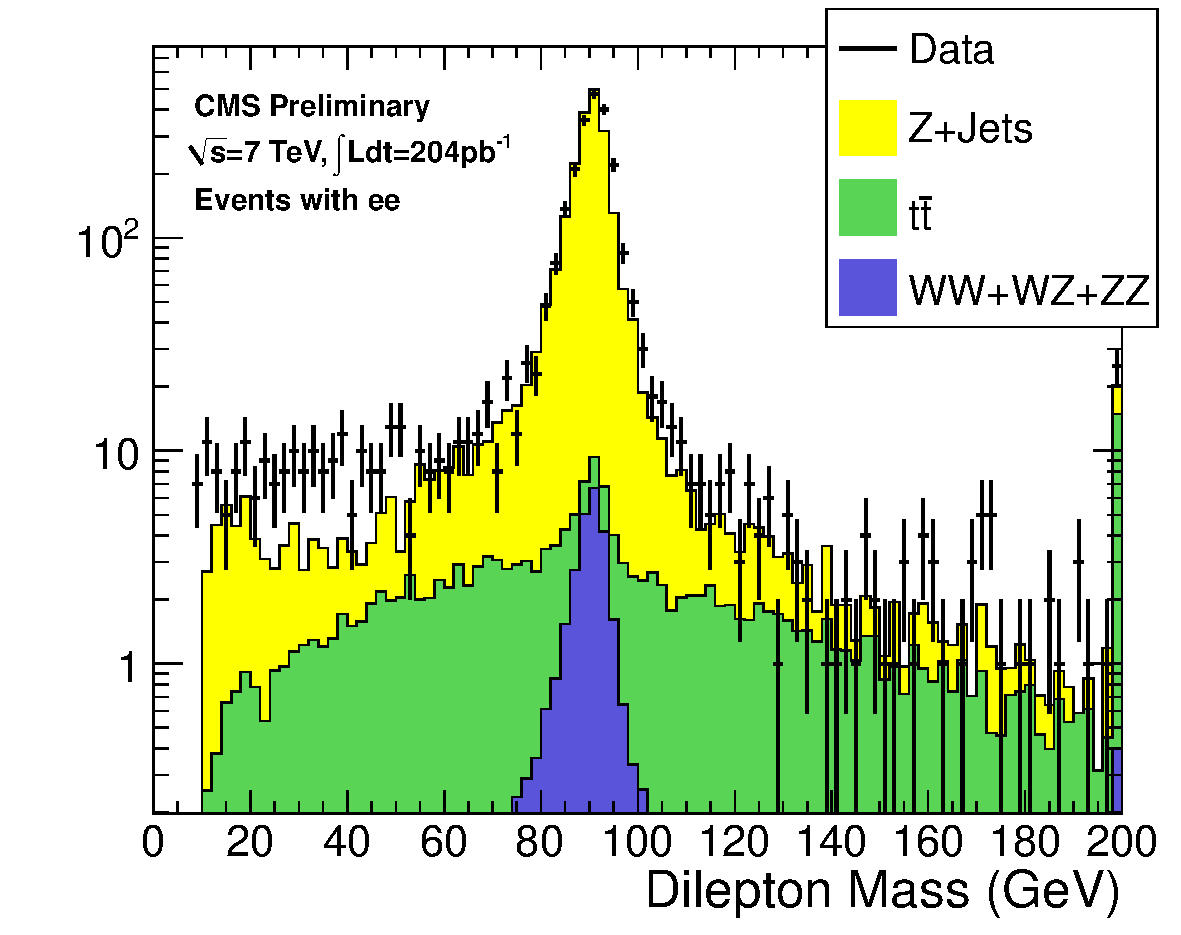
\includegraphics[width=0.48\linewidth]{plots/hdilmass_ee_allj.pdf}
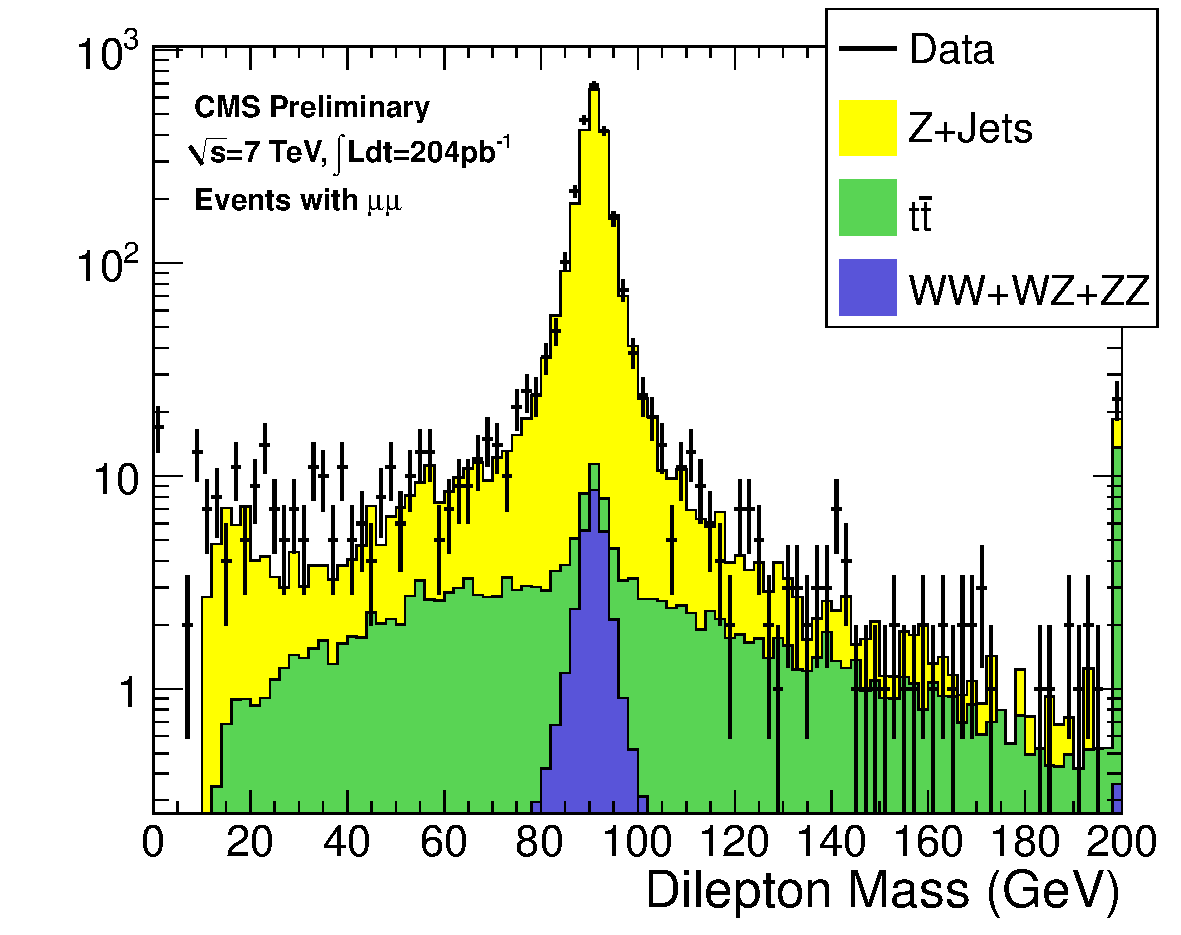
\includegraphics[width=0.48\linewidth]{plots/hdilmass_mm_allj.pdf}
\caption{\label{fig:dilmass}\protect Dilepton mass distribution for events passing the pre-selection
  in the $ee$ (left) and $\mu\mu$ (right) final states. Backgrounds from single top and $W$+jets are omitted
  since they are negligible.}
\end{center}
\end{figure}

\begin{table}[htb]
\begin{center}
\caption{\label{preselyieldtable} Data and MC yields passing preselection.
The MC uncertainties are statistical only.
}
\begin{tabular}{lccccc}
\hline
sample     &            $ee$   &        $\mu\mu$   &       $e\mu$   &              tot  \\
\hline
\zjets     & 1840.6 $\pm$ 21.2 & 2088.0 $\pm$ 22.6 &  1.5 $\pm$ 0.6 & 3930.1 $\pm$ 31.0 \\
\ttbar     &   24.5 $\pm$  0.9 &   26.0 $\pm$  0.9 & 51.3 $\pm$ 1.2 &  101.8 $\pm$ 1.8  \\
\wjets     &    0.9 $\pm$  0.6 &    0.0 $\pm$  0.0 &  0.4 $\pm$ 0.4 &    1.3 $\pm$ 0.7  \\
\WW        &    0.2 $\pm$  0.0 &    0.4 $\pm$  0.1 &  0.6 $\pm$ 0.1 &    1.3 $\pm$ 0.1  \\
\WZ        &   13.9 $\pm$  0.2 &   16.0 $\pm$  0.2 &  0.1 $\pm$ 0.0 &   30.1 $\pm$ 0.2  \\
\ZZ        &   10.0 $\pm$  0.1 &   11.4 $\pm$  0.1 &  0.0 $\pm$ 0.0 &   21.4 $\pm$ 0.1  \\
single top &    0.7 $\pm$  0.1 &    0.8 $\pm$  0.1 &  1.7 $\pm$ 0.1 &    3.2 $\pm$ 0.1  \\
\hline
total MC   & 1890.8 $\pm$ 21.2 & 2142.6 $\pm$ 22.6 & 55.6 $\pm$ 1.4 & 4089.0 $\pm$ 31.1 \\
\hline
      data &   2051            &    2277           &      66        &    4394           \\ 
\hline
\end{tabular}
\end{center}
\end{table}

Samples of  MC events are used to  guide the  design of  the analysis.
These      events     are      generated     using      either     the
\PYTHIA6.4.22~\cite{Pythia}  or  \MADGRAPH4.4.12~\cite{Madgraph} event
generators.    They   are   then   simulated  using   a   GEANT4-based
model~\cite{Geant} of the CMS  detector, and finally reconstructed and
analyzed using the same software as is used to process collision data.

Events with     two     opposite-sign,     isolated    leptons     ($e^+e^-$,
$e^{\pm}\mu^{\mp}$, or $\mu^+\mu^-$) are selected. Both leptons must have
\pt $>$ 20\GeVc and the electrons (muons) must have $|\eta| < 2.5$ ($|\eta| < 2.4$). In events
with more  than two such leptons,   the two  leptons with invariant mass
closest to the $Z$ mass are selected. The leptons are required to be
consistent with originating from the $Z$ by requiring the invariant
mass to satisfy $81 < \mathrm{M(\ell\ell)} < 101$\GeVcc.

Events are required to pass  at least one  of a set of $ee$, $e\mu$ or $\mu\mu$
double-lepton triggers.  The  efficiency for events containing two 
leptons passing the analysis selection to  pass at  least  one of  these
triggers  is measured to be approximately 100\%, 95\%, and 90\%
for $ee$, $e\mu$ or $\mu\mu$ double-lepton triggers, respectively.
In the following, the MC yields are weighted by these trigger efficiencies.

Because leptons produced in the  decays of low-mass particles, such as
hadrons containing $b$  and $c$ quarks,  are  nearly  always inside  jets,  they can  be
suppressed by requiring the leptons to be isolated in space from other
particles that carry a  substantial amount of transverse momentum. The
details   of   the  lepton   isolation   measurement   are  given   in
Ref.~\cite{ref:top}.   In  brief,   a cone is constructed     of  size
$\Delta{}R\equiv\sqrt{(\Delta\eta)^2+(\Delta\phi)^2}=0.3$  around  the
lepton  momentum  direction. The  lepton  relative  isolation is  then
quantified  by  summing the  transverse  energy  (as  measured in  the
calorimeters) and the transverse  momentum (as measured in the silicon
tracker) of  all objects  within this cone,  excluding the  lepton, and
dividing by  the lepton transverse momentum. The resulting quantity
is required to be  less than 0.15, rejecting
the large background arising from QCD production of jets.

We require the presence of at least two jets with  $\pt > 30\GeVc$ and  $|\eta| < 3.0$,
separated  by $\Delta  R  >$  0.4 from  leptons  passing the  analysis
selection.    The  anti-$k_T$   clustering
algorithm~\cite{antikt}  with  $\Delta{}R  =  0.5$  is  used  for  jet
clustering. The jets and MET  are reconstructed with the Particle Flow 
technique~\cite{CMS-PAS-PFT-10-002}. 
 
The resulting dilepton mass spectra for the $ee$ and $\mu\mu$ final states for events
passing the above requirements except for the $Z$ mass requirement are shown in Figure~\ref{fig:dilmass}.
The data and MC yields passing the full preselection above are displayed in Table~\ref{preselyieldtable}.
The MC yields are normalized to \lumi, assuming 100\% trigger efficiency. 
As anticipated, the MC predicts that the preselection is dominated by \zjets\ in the same-flavor 
case and by \ttbar\ in the opposite-flavor case.  
The data yield is in reasonable agreement with the predictions for the $ee$, $\mu\mu$ and $e\mu$ channels.
